% Created 2017-09-22 Fri 00:18
% Intended LaTeX compiler: pdflatex
\documentclass[a4paper]{scrartcl}
\usepackage[utf8]{inputenc}
\usepackage[T1]{fontenc}
\usepackage{graphicx}
\usepackage{grffile}
\usepackage{longtable}
\usepackage{wrapfig}
\usepackage{rotating}
\usepackage[normalem]{ulem}
\usepackage{amsmath}
\usepackage{textcomp}
\usepackage{amssymb}
\usepackage{capt-of}
\usepackage{hyperref}
\usepackage{indentfirst}
\setlength{\parindent}{2em}
\setlength{\parskip}{1em}
\hypersetup{hidelinks=true}
\author{Hu Xiaoxiang \\
U1521319A \\
EEE \\
}
\date{Sep 21, 2017 \\
}
\title{
\includegraphics[width=\textwidth]{logo_ntu_new.png} \\
[3\baselineskip] ASSIGNMENT \\
REPORT \\
[7\baselineskip]}
\hypersetup{
 pdfauthor={Hu Xiaoxiang \\
U1521319A \\
EEE \\
},
 pdftitle={
\includegraphics[width=\textwidth]{logo_ntu_new.png} \\
[3\baselineskip] ASSIGNMENT \\
REPORT \\
[7\baselineskip]},
 pdfkeywords={},
 pdfsubject={},
 pdfcreator={Emacs 25.1.1 (Org mode 9.1.1)}, 
 pdflang={English}}
\begin{document}

\maketitle
\tableofcontents

\newpage
\section{Algorithm Description}
\label{sec:org74dd27f}
\subsection{Bisection method}
\label{sec:org4a0bc4b}
The bisection method in mathematics is a root-finding method that repeatedly
bisects an interval and then selects a subinterval in which a subinterval
in which a root must lie for further processing.
\subsection{Newton-Raphson method}
\label{sec:orgf99cf3b}
The Newton-Raphson method is a method for finding successively better
approximations to the roots of a real-valued function. The formula of
Newton-Raphson method is $$x_{n+1} = x_n - \frac{f(x_n)}{f'(x_n)}$$

\section{Proof}
\label{sec:orgd1faf02}
\subsection{Bisection method}
\label{sec:org02a362d}
Firstly I assume the given number \(X_0\) is positive. Because the symmetry of
the positive and negative number on number axis, the algorithm should work
for negative number as long as it works for positive number.

I. If \(x_0 > 1\), let \(x_{high_0} = x_0\), \(x_{low_0} = 0\), \(x_{mid_0} = \frac{x_{high_0} + x_{low_0}}{2}\)
\begin{center}
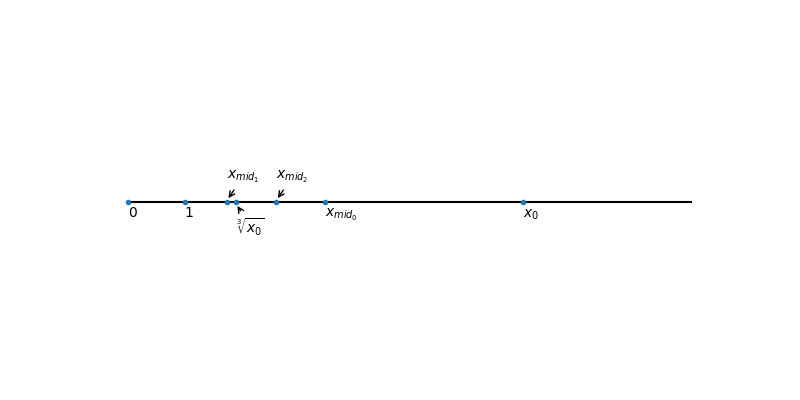
\includegraphics[width=.9\linewidth]{numberAxis1.png}
\end{center}

Step A: If \(x^3_{mid_0} > x_0 \Rightarrow x_{mid_0} > \sqrt[3]{x}\),

then let \(x_{high_1} = x_{mid_0}\), \(x_{low_1} = x_{low_0} = 0\), \(x_{mid_1} = \frac{x_{high_1} + x_{low_1}}{2}\)

Step B: If \(x^3_{mid_1} < x_0 \Rightarrow x_{mid_1} < \sqrt[3]{x}\),

then let \(x_{low_2} = x_{mid_1}\), \(x_{high_2} = x_{high_1} = x_{mid_0}\), \(x_{mid_2} = \frac{x_{high_2} + x_{low_2}}{2}\)

Repeat step A or B until \(|x_{mid_{n+1}} - x_{mid_n}| < precision~error\)

II. If \(x_0 < 1\), let \(x_{high_0} = 1\), \(x_{low_0} = x_0\), \(x_{mid_0} = \frac{x_{high_0} + x_{low_0}}{2}\)
\begin{center}
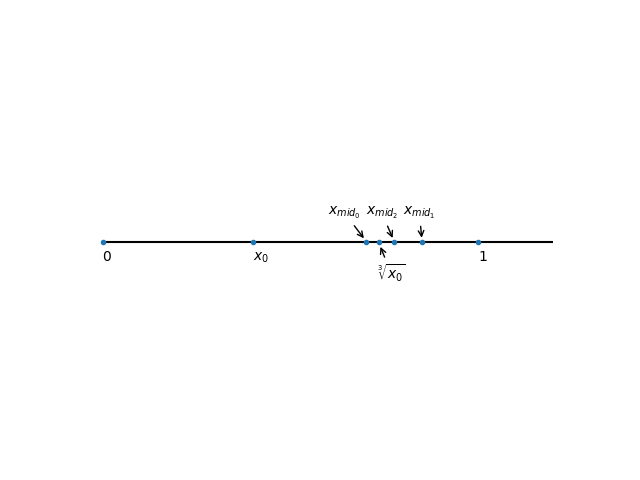
\includegraphics[width=.9\linewidth]{numberAxis2.png}
\end{center}

Step A: If \(x^3_{mid_0} < x_0 \Rightarrow x_{mid_0} < \sqrt[3]{x}\),

then let \(x_{low_1} = x_{mid_0}\), \(x_{high_1} = x_{high_0} = 1\), \(x_{mid_1} = \frac{x_{high_1} + x_{low_1}}{2}\)

Step B: If \(x^3_{mid_1} > x_0 \Rightarrow x_{mid_1} > \sqrt[3]{x}\),

then let \(x_{high_2} = x_{mid_1}\), \(x_{low_2} = x_{low_1} = x_{mid_0}\), \(x_{mid_2} = \frac{x_{high_2} + x_{low_2}}{2}\)

Repeat step A or B until \(|x_{mid_{n+1}} - x_{mid_n}| < precision~error\)

\subsection{Newton-Raphson method}
\label{sec:org59fddc5}
\begin{center}
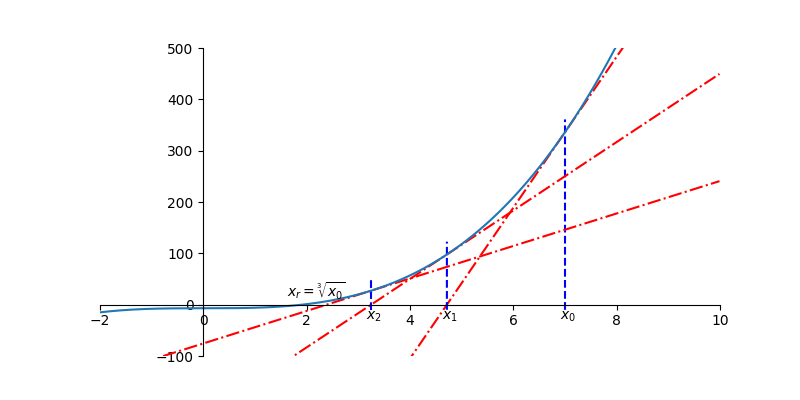
\includegraphics[width=.9\linewidth]{numberAxis3.png}
\end{center}

Let \(x_r = \sqrt[3]{x_0}\), so \(f(x_r) = 0 ~~-------------------------~Eq.1\)

Given \(x_{n+1} = x_n - \frac{f(x_n)}{f'(x_n)} ~~-----------------------~Eq.2\)

By Taylor Series,
$$f(x_r) = f(x_n) + f'(x_n)(x_r - x_n) + \frac{f''(x_n)}{2!}(x_r-x_n)^2 + \frac{f'''(x_n)}{3!}(x_r-x_n)^3+\cdots$$

Here the previous three items are used as the dominant polynomials.

Let \(f(x_r) \approx f(x_n) + f'(x_n)(x_r - x_n) + \frac{f''(x_n)}{2!}(x_r-x_n)^2 ~~-----------~Eq.3\)

Substitute Eq.1 and Eq.2 into Eq.3,

\(\Rightarrow 0 = f'(x_n)(x_n - x_{n+1}) + f'(x_n)(x_r - x_n) + \frac{f''(x_n)}{2!}(x_r-x_n)^2\)

\(\Rightarrow x_{n+1} - x_r = \frac{f''(x_n)}{2!}(x_r-x_n)^2\)

Let error \(e_n = x_n -x_r\),

\(\Rightarrow e_{n+1} = \frac{f''(x_n)}{2f'(x_n)}e^2_n ~~-----------------------------~Eq.4\)

The last equation shows that after each iteration, the error in new estimate
is proportional to the square of the old estimate. That means the precision
digits will double for each iteration.

\section{Complexity Analysis}
\label{sec:orgda7b128}

\subsection{Bisection method}
\label{sec:org5d6b0b0}
Here I define the time complexity is dependent on the required precision
digit N. For example, 1.12345 with precision digit N=3 means the first 3
digits after decimal point .123 are accurate.

Considering the worst case, to determine one precision digit, for example,
the current state is \(x_{low_0} = 1.0\), \(x_{high_0} = 2.0\) and the expected
first accurate digit is 1.1. By definition \(x_{mid_n} = \frac{x_{high_n} +
   x_{low_n}}{2}\), we can find \(x_{mid_0} = 1.5\). After several iterations we
can get \(x_{mid_1} = 1.25\), \(x_{mid_2} = 1.125\), \(x_{mid_3} = 1.0625\),
\(x_{mid_4} = 1.09375\), \(x_{mid_5} = 1.109375\).

This shows that the algorithm needs to iterate at most 6 times to determine
the interval where the accurate digit lies for the worst case. If the
required precision digits is N, then it needs at most 6N times to find the
required precision interval, which means the time complexity of bisection
method is \(O(N)\).

\subsection{Newton-Raphson method}
\label{sec:orgbad55a3}
The Eq.4 \(e_{n+1} = \frac{f''(x_n)}{2f'(x_n)}e^2_n\) shows that the precision
digits will double after each iteration. For example, if the error for the
1st time iteration is 0.1(N=1), the error for the 2nd and 3rd time iteration
will be 0.1\(^{\text{2}}\) = 0.01(N=2) and 0.0001(N=2\(^{\text{2}}\)). So after t times of iteration,
the precision digits is proportional to the square of t: \(N \propto 2^t\). If
ignoring the affect of the initial value \(x_0\), the time complexity of
Newton-Raphson method is \(O(\log_2 N)\)

\section{Conclusion}
\label{sec:org6745239}
After several times of experiment, the results show that with the increasing
number of precision digits N, the total number of iterations for
bisection method is proportional to N. 

For Newton-Raphson method, the number of iterations does not increase
significantly, which verifies its complexity is proportional to \(\log_2 N\).
However, the Eq.4 shows that the error of next iteration is also dependent on
the previous input value \(x_n\), which means the initial value has a
significant influence on the time complexity of Newton-Raphson method. Since
it is impossible to determine the optimal value for \(x_0\), we cannot
explicitly define the time complexity of Newton-Raphson method.
\end{document}
